\section{Implementation}\label{implement}

The following chapter describes the implementation of the project. Figure \ref{fig:pipeline} shows the pipeline of the application.

\begin{figure}[H]
    \centering
    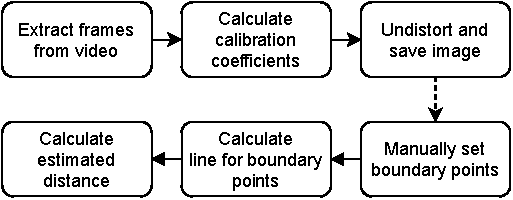
\includegraphics[width=.7\textwidth]{image/2/pipeline.pdf}
    \caption{Pipeline}
    \label{fig:pipeline}
\end{figure}
The pipeline consists of two components: The camera calibration and the manual calculation of the estimated distance. Since a segmentation or a mask from the checkerboard would be necessary to automatically calculate the estimated distance, the creation of the boundary points and the calculation of the estimated distance is done manually.\\

This pipeline will be demonstrated on the basis of figure \ref{fig:250_ref_og} in recording \textit{'250\_cm\_distance.h264'}, where the distance to the object is known to be 250cm.

\begin{figure}[H]
    \centering
    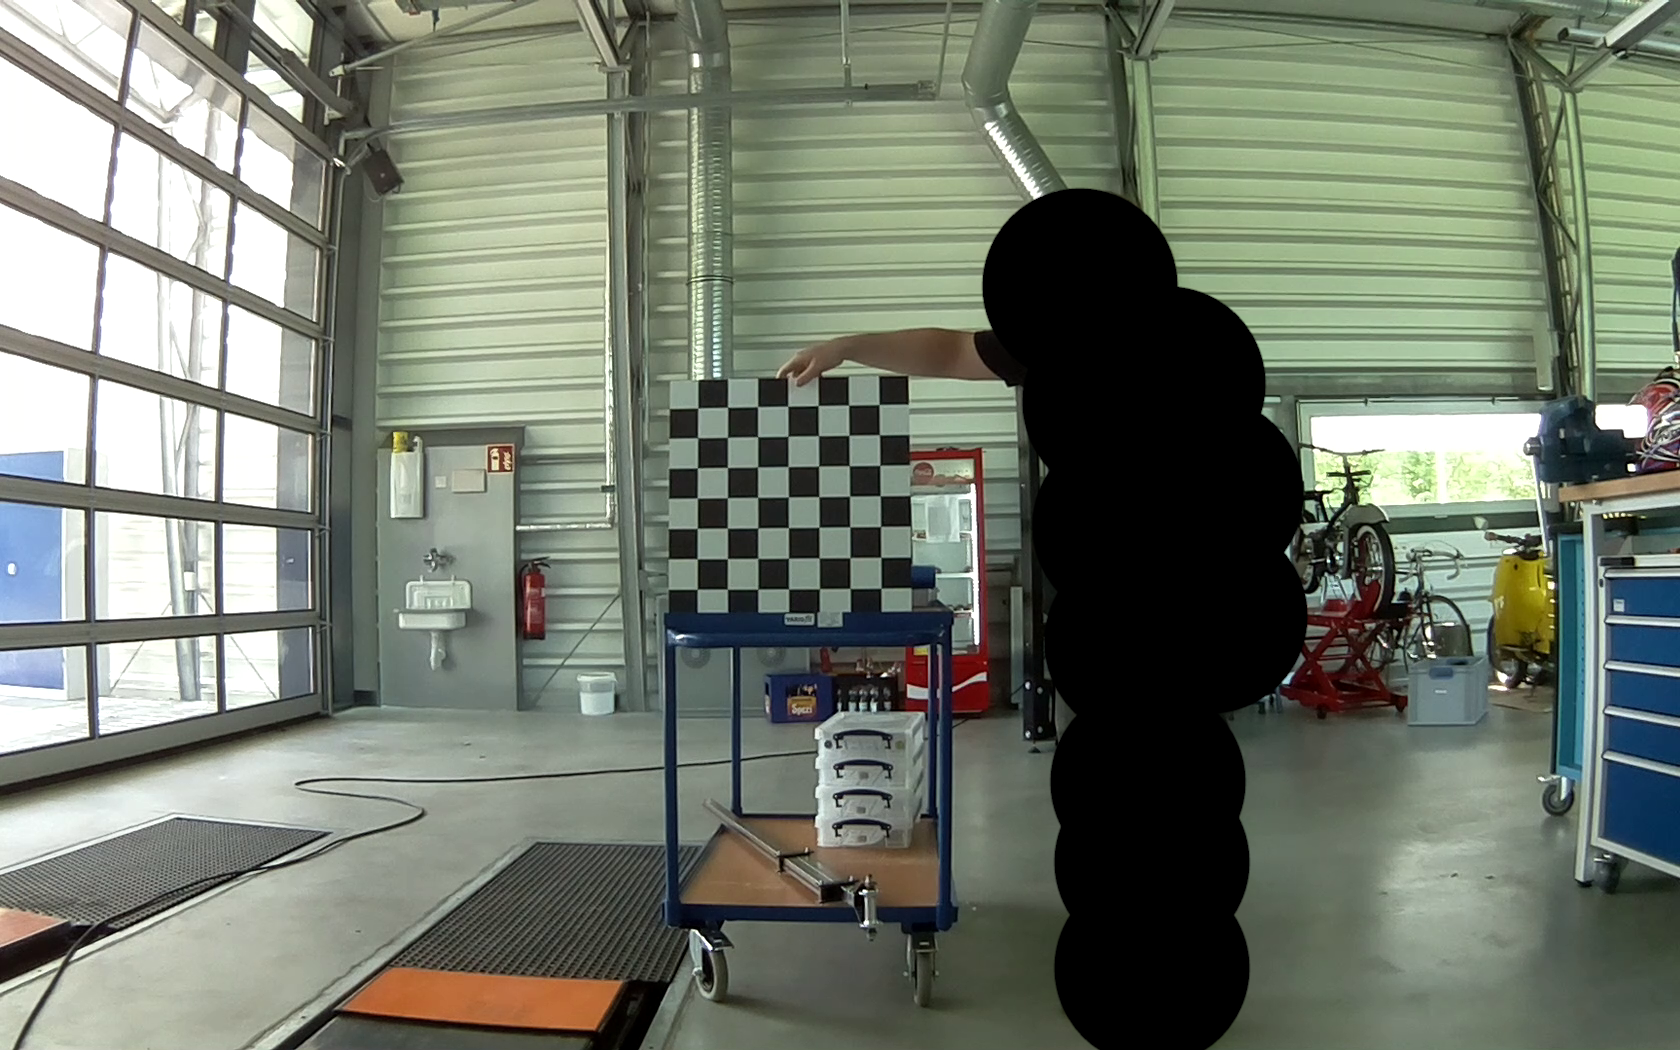
\includegraphics[width=.7\textwidth]{image/2/250_ref_og.png}
    \caption{Original frame from the source recording}
    \label{fig:250_ref_og}
\end{figure}

\newpage
\vspace{-2em}
\subsection{Intrinsic Matrix}

The algorithm starts to read in all frames from a recording. If the frames of the recording can be accessed, they are processed successively to find the interior corners of the checkerboard in the frames with a specified corner size. A preprocessing step is taken beforehand which downscales the original 1920x1080 frame to a smaller resolution to cutoff processing time. If a checkerboard is found, this frame is saved separately.\\

In this step, however, the intrinsic matrix is not calculated. Only images where the checkerboard was successfully found with a specified corner size are saved. It is necessary to sort the images to avoid duplicates and non-unique images before the intrinsic matrix is calculated.\\

One possibility would be to calculate the intrinsic matrix with all frames where a checkerboard with known corner size was successfully found. However, this has the consequence that the calculation of the intrinsic matrix takes more processing time. Furthermore there is no merit in using images where no new or unique information about the image appears. Therefore the number of images for the calibration should be as small as possible with as much unique information as possible.\\
That is why in this project the images are sorted manually. It is recommended to use at least "10 images of a 7 × 8 or larger chessboard" \cite{cv} to obtain high-quality results \cite{cv}\\

The selection of the images that form the basis of the calibration of the intrinsic matrix is particularly crucial. Depending on which images are used, they can strongly influence the coefficients of the intrinsic matrix and thus the estimated distance. This poses a potential danger.\\ % corner size

After the best images have been selected from the set of frames, they can now be used to calculate the intrinsic matrix and distortion coefficients. For this purpose, the methodology in \cite{zhang2000} will be used. Additionally the distortion matrix needs to be calculated too. The methodology for this is described in \cite{brown} and \cite{brown_2}. \cite{cv}\\
When both sets of coefficients are acquired the distorted image can be undistorted. For this purpose, the methodology described in \cite{distort_cv} is used.\\

% Enforce Text on same page (no page break)
\begin{minipage}{\textwidth}
To further improve the coefficients of the intrinsic matrix, the undistorted images can be undistorted again.
\end{minipage}

\newpage
\subsection{Distance Estimation}

After the intrinsic matrix for the recording has been calculated, the approximate distance to the object can now be calculated with the assumptions made in chapter \ref{obj}. However, this is only an estimated distance, since the coefficients of the intrinsic matrix are subjected to noise depending on the recordings and the used images for the calibration.\\

To do this, an image is first created that clearly shows the object in the desired distance with the object. In this case the last frame of the \textit{'250\_cm\_distance.h264’}-recording was taken and an undistorted image was generated from it with the calculated intrinsic matrix and distortion coefficients. The result can be seen in figure \ref{fig:250_og}.\\

From this image, two boundary points are now determined that lie on the edge of the checkerboard and on a straight line. The boundary points are marked as green points in figure \ref{fig:250_green}. In the same process the pixel coordinates $(z_1, z_2)^{T}$ can be noted for both boundary points.\\

\begin{figure}[H]
     \centering
     \captionsetup{justification=centering}
     \begin{minipage}[t]{0.5\textwidth}
        \centering
        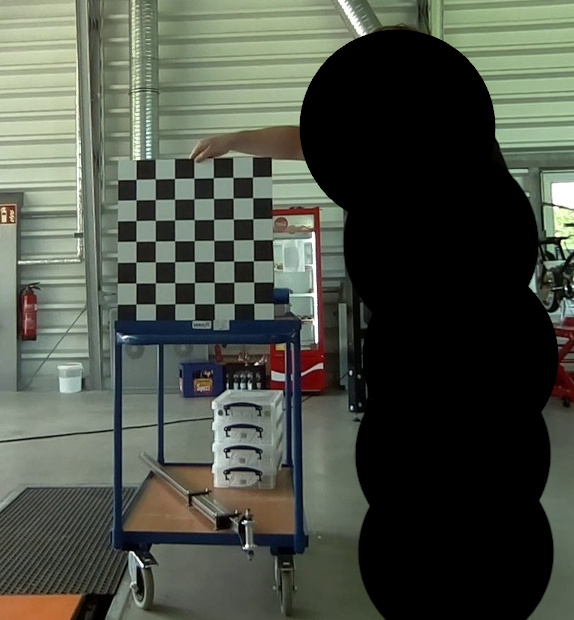
\includegraphics[width=.95\textwidth]{image/2/250_undist_cropped.jpg}
        \caption{Undistorted and cropped image}
        \label{fig:250_og}
     \end{minipage}%
     \begin{minipage}[t]{0.5\textwidth}
        \centering
        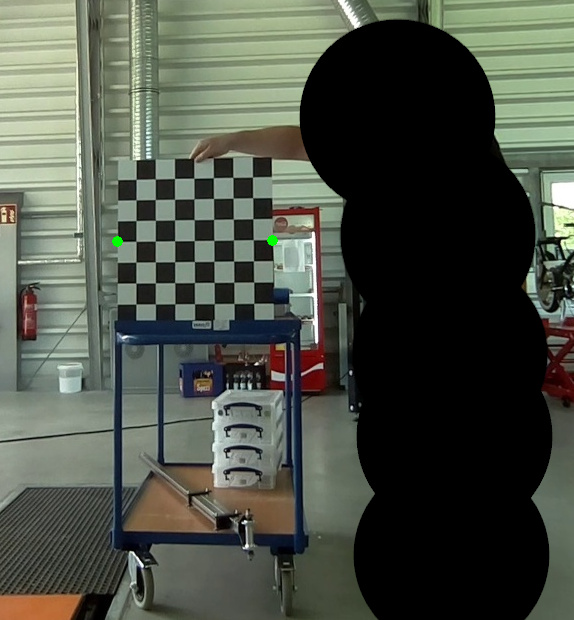
\includegraphics[width=.95\textwidth]{image/2/250_undist_cropped_green.jpg}
        \caption{Boundary points \textit{A} and \textit{B} \\in green colour}
        \label{fig:250_green}
     \end{minipage}
\end{figure}

\newpage 
With the pixel coordinates $(z_1, z_2)^{T}$ and the intrinsic matrix $\bm{K}$ one can calculate the \\ simplified full line $\vec{L}$ between camera and pixel coordinate. The equation can be seen in equation \ref{eq:1}. The calculated line $z \vec{\lambda}$ is filled with potential distance positions $z$.

{\large
\begin{equation}\label{eq:1}
    \vec{L} = \left \{ 
            \begin{pmatrix}
                \lambda_1\\ 
                \lambda_2\\ 
                \lambda_3
            \end{pmatrix} 
            \in \mathbb{R}^{3}\text{;}\;
            z \! \begin{pmatrix}
                \lambda_1\\ 
                \lambda_2\\ 
                \lambda_3
            \end{pmatrix} 
            = z\bm{k}
            \begin{pmatrix}
                z_1\\ 
                z_2\\ 
                1
            \end{pmatrix} 
            \text{and} \; z \in \mathbb{R}\right \}
            \text{with} \; \bm{k} = \bm{K^{-1}}
\end{equation}
}
\vspace{2mm}

%\newpage

With the equation \ref{eq:1} and the known boundary points \textbf{A} and \textbf{B} with pixel coordinates $(z_1, z_2)^{T}$ one can calculate the corresponding vectors $\vec{a}$ and $\vec{b}$ shown in equation \ref{eq:2_1} and \ref{eq:2_2}.

{\large
\begin{align}\label{eq:2_1}
    \vec{a}(z) &= z \vec{\lambda_A} = z \! 
    \begin{pmatrix}
        \lambda_{1A}\\ 
        \lambda_{2A}\\ 
        \lambda_{3A}
    \end{pmatrix} = z\bm{k}
    \begin{pmatrix}
        A_x\\ 
        A_y\\
        1
    \end{pmatrix} = z\bm{k}
    \begin{pmatrix}
        z_{1A}\\ 
        z_{2A}\\
        1
    \end{pmatrix}\\[10pt]
    \vec{b}(z) &= z \vec{\lambda_B} = z \! 
    \begin{pmatrix}
        \lambda_{1B}\\ 
        \lambda_{2B}\\
        \lambda_{3B}
    \end{pmatrix} = z\bm{k}
    \begin{pmatrix}
        B_x\\ 
        B_y\\
        1
    \end{pmatrix}= z\bm{k}
    \begin{pmatrix}
        z_{1B}\\ 
        z_{2B}\\
        1
    \end{pmatrix}\label{eq:2_2}
\end{align}
}

\begin{wrapfigure}[19]{L}{0.57\textwidth}
    \vspace{\baselineskip}
    \centering
     \captionsetup{justification=centering}
     \begin{minipage}[b]{0.55\textwidth}
         \centering
         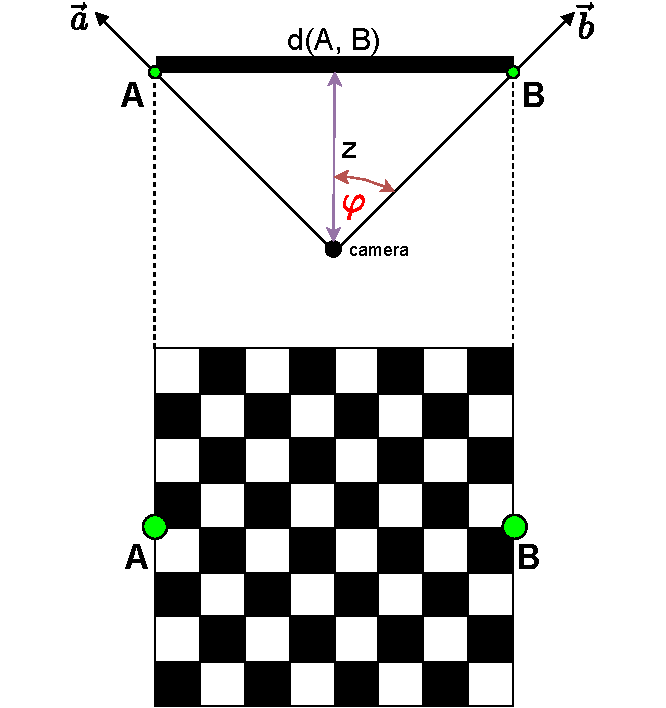
\includegraphics[width=\textwidth]{image/2/calc_line.pdf}
         \caption{Visualisation of the relationships}
         \label{fig:calc_line}\par
     \end{minipage}

\end{wrapfigure}

\newpage
These relationships are shown again in figure \ref{fig:calc_line}. \\The vectors $\vec{a}$ and $\vec{b}$ and the known size of the checkerboard $d(A, B)$ are defining a triangular area based on the assumptions  made in chapter \ref{obj}. \\

Since one assumption is that the checkerboard is perpendicular to the camera, we can assume that the vectors $\vec{a}$ and $\vec{b}$ have the same angle to the camera. Thus we can calculate the distance $z$ of the resulting triangle if the norms $|\vec{a}(z)|=|\vec{b}(z)|$ with a distance between the vectors of $d(A, B)$. For this one can use the trigonometric formulas if the angle between both vectors is known.\\

The angle $\varphi_{tot}$ between two vectors can be calculated using the dot product.
\vspace{-2mm}
{\large % change font size
% https://de.overleaf.com/learn/latex/Spacing_in_math_mode
\begin{align}
    \varphi_{tot} &= \arccos{\frac{\vec{a} \cdot \vec{b}}{|\vec{a}||\vec{b}|}}\nonumber\\[5pt]
    \varphi_{tot} &= 2\varphi = \arccos{\frac{\vec{\lambda_A} \cdot \vec{\lambda_B}}{|\vec{\lambda_A}||\vec{\lambda_B}|}}\nonumber\\[5pt]
    \Rightarrow \varphi &= \frac{1}{2}\arccos{\frac{\vec{\lambda_A} \cdot \vec{\lambda_B}}{|\vec{\lambda_A}||\vec{\lambda_B}|}}\label{eq3}
    % d(A, B)^{2} &= (z \lambda_{1A} - z \lambda_{1B})^{2} + (z \lambda_{2A} - z \lambda_{2B})^{2}\\
    % d(A, B)^{2} &= z^{2}(kA_x - kB_x)^{2} + z^{2}(kA_y - kB_y)^{2}\\
    % d(A, B)^{2} &= z^{2}[(\overset{\thicksim}{A_x} - \overset{\thicksim}{B_x})^{2} + \overset{\thicksim}{A_y} - \overset{\thicksim}{B_y})^{2}]
\end{align}
}

\newpage

With the calculated angle $\varphi$ one can calculate the distance $z$ using the trigonometric formulas. 
{\large
\begin{align}
    \tan{\varphi} &= \frac{\frac{d(A, B)}{2}}{z}\nonumber\\
    \Rightarrow z &= \frac{d(A, B)}{2\tan{\varphi}}\label{eq4}
    % (50cm)^{2} &= z^{2}\cdot x \nonumber\\
    % z &= \sqrt{\frac{(50)^2}{x}}\;cm \label{eq3}
\end{align}
}

With the intrinsic matrix $\bm{K}$, the boundary points \textbf{A} and \textbf{B}, the known size of the checkerboard $d(A, B)$ and the equations \ref{eq:2_1}, \ref{eq:2_2}, \ref{eq3} and \ref{eq4} one can calculate the estimated distance $z$ between camera and object.







\subsection{Printer size estimation}

\begin{wrapfigure}[15]{L}{0.5\textwidth}
    \vspace{-.75\baselineskip}
    \centering
     \captionsetup{justification=centering}
     \begin{minipage}[b]{0.45\textwidth}
         \centering
         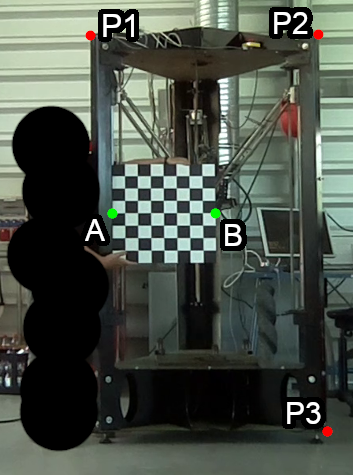
\includegraphics[width=\textwidth]{image/2/metal_printer_size.png}
         \caption{Marked pixel coordinates}
         \label{fig:printer_size}\par
     \end{minipage}
\end{wrapfigure}

Furthermore, we can measure the size of objects at the same distance as a reference object. In this project, the width and height of the 3D metal printer is to be determined. This can be seen in figure \ref{fig:printer_size}.\\

For this purpose the boundary points with pixel coordinates $(z_1, z_2)^{T}$ of the known reference object are marked, just like the corner points of the searched for object. In this example the boundary of the checkerboard are marked with green points and the corner points of the 3D metal printer are marked with red points.

\newpage
The boundary points of the checkerboard should lie on the edge of the checkerboard and on a straight line as that is where the known distance $d(A, B)$ lies. Since the checkerboard has edges of equal length, we can assume the same distance for the height as for the width. Therefore only two boundary points are needed.\\ 

With the pixel coordinates $\bm{A, B, P_1, P_2, P_3}$ one can now calculate the size of the 3D metal printer. For this purpose, the ratio of the norm between two points and the norm between the boundary points is calculated and scaled with the reference distance.

\begin{align}
    width &= \frac{|\bm{P1}-\bm{P2}|}{|\bm{A}-\bm{B}|}\cdot d(A, B)\label{eq5}\\[10pt]
    height &= \frac{|\bm{P2}-\bm{P3}|}{|\bm{A}-\bm{B}|}\cdot d(A, B)\label{eq6}
\end{align}
